\usetikzlibrary{shapes}
\usetikzlibrary{arrows}
\usetikzlibrary{calc,positioning}
\begin{figure}
\centering
\scalebox{0.9}{
	\scriptsize
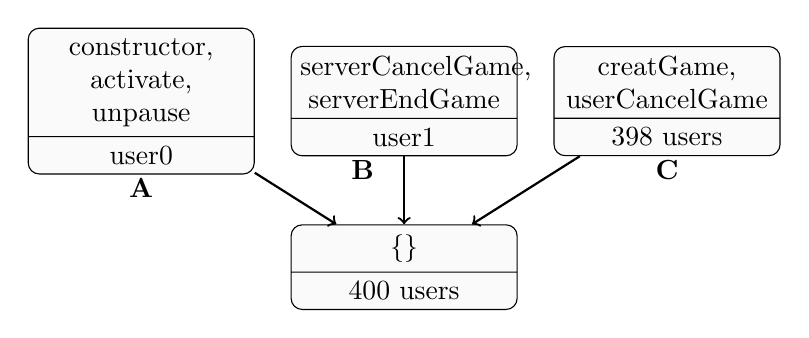
\begin{tikzpicture}%	[edge from parent path=
%	{(\tikzparentnode.north) .. controls +(0,1) and +(0,-1)
%		.. (\tikzchildnode.south)}]
	\tikzstyle{role}=[fill={rgb:black,1;white,50}, draw, rounded corners,
	rectangle split,  
	rectangle split parts=2, 
	rectangle split draw splits=true,  text centered, text width=75]
	\tikzstyle{edge from parent}=[black,<-,thick,draw]
	\node[role] (root) { \{\}  \nodepart{two} 400 users } [level distance = 60, sibling distance=95, grow=up]
	child {node[role] (roleC) {creatGame, userCancelGame \nodepart{two} 398 users }}
	child {node[role] (roleB) {serverCancelGame, serverEndGame  \nodepart{two} user1}}
	child {node[role] (roleA) {constructor, activate, unpause  \nodepart{two} user0}
	};
	\draw ([yshift=-5pt]roleA.south) node[] {\textbf{A}};
	\draw ([yshift=-5pt, xshift=-15pt]roleB.south) node[] {\textbf{B}};
	\draw ([yshift=-5pt]roleC.south) node[] {\textbf{C}};
\end{tikzpicture}
}
\caption{The roles of Dicether.}
\label{fig: DicetherRole}
\end{figure}